\begin{enumerate}[(a)]
  \item
        \q{Ecrire une fonction }\il{temps(n)}\q{ qui renvoie le rapport des temps
          $\frac{t_i(n)}{t_r(n)}$ pour une même liste $T_0$ de $n$ nombres aléatoires
          entiers où $t_i(n)$ est le temps du tri par insertion et $t_r(n)$ le temps du
          tri rapide. }

        \codeFromFileT{exercices.py}{section-02/q1/1.py}

  \item \q{Vérifier que $10\leq$ }\il{temps(1000)}\q{ $\leq20$}\\
        \il{print(temps(1000))} donne : \il{15.828425459447944}
  \item \q{Vérifier graphiquement en faisant varier $n$ dans l’ensemble}
        \il{np.array([300,700,800,1000,1500,2000])}
        \q{qu’on a la relation : $\frac{t_i(n)}{t_r(n)} \underset{+\infty}{\sim}
            C \frac{n}{ln(n)}$ et donner la valeur de la constante $C$.}

        \codeFromFileT{exercice.py}{section-02/q1/2.py}
        Mais lorsque j'exécute \il{graphe()}, je n'obtiens pas une droite\dots
        même en répétant l'opération\dots
        \begin{center}
          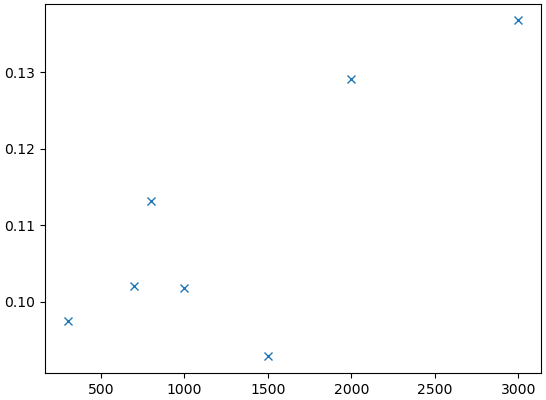
\includegraphics[scale=0.5]{section-02/q1/3.png}
        \end{center}

\end{enumerate}
